\chapter{\IfLanguageName{dutch}{Voorstelling van skills en draaierstrucs}{Display of skills and turners}}%
\label{ch:skills and turners}


In this appendix, skills will be displayed to give an example what exactly needs to be recognized. The focus of the first section is showing some subdisciplines of jump rope. The second part involves displaying performed skills and turners in Double Dutch.

\section{Jump Rope Disciplines}
\label{subsubsec:jump-rope-disciplines}

This section will focus on showing images of subdisciplines to make clear what entails each discipline.

\begin{figure}
    \centering
    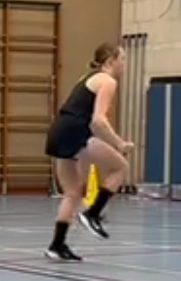
\includegraphics[width=0.32\linewidth]{sr-speed-c}
    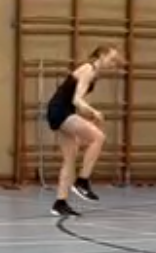
\includegraphics[width=0.32\linewidth]{sr-speed-le}
    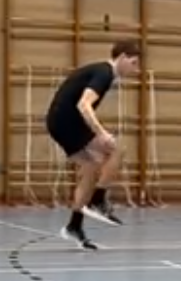
\includegraphics[width=0.32\linewidth]{sr-speed-m}
    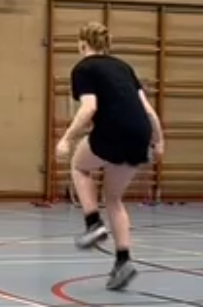
\includegraphics[width=0.4\linewidth]{sr-speed-lo}
    \label{fig:sr-speed-c}
    \caption[Jumpers performing single rope speed]{Jumpers performing single rope speed.}
\end{figure}

\begin{figure}
    \centering
    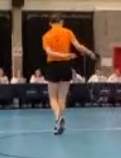
\includegraphics[width=0.4\linewidth]{sr.png}
    \caption[Athlete in a Single Rope routine]{Athlete in a Single Rope routine doing a wrap.}
    \label{fig:sr-wrap}
\end{figure}




\begin{figure}
    \centering
    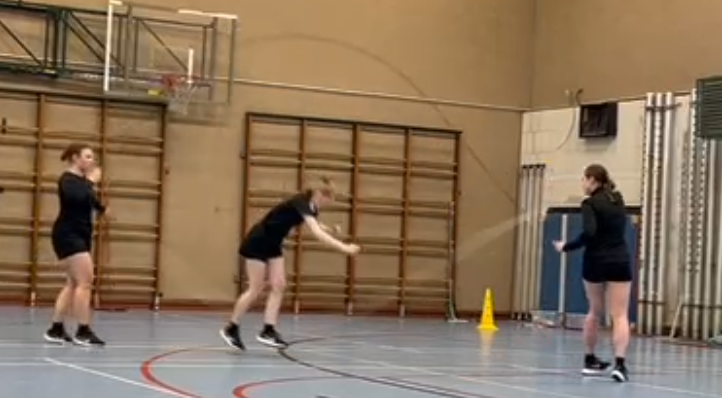
\includegraphics[height=0.14\linewidth]{dd3-du-flip-ts-1}
    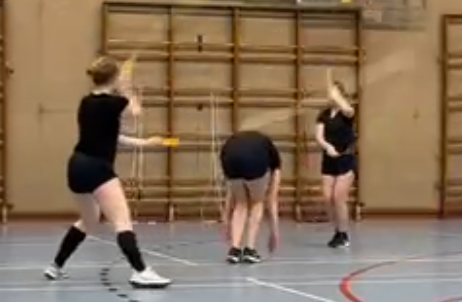
\includegraphics[height=0.14\linewidth]{dd3-du-crab-cross-1}
    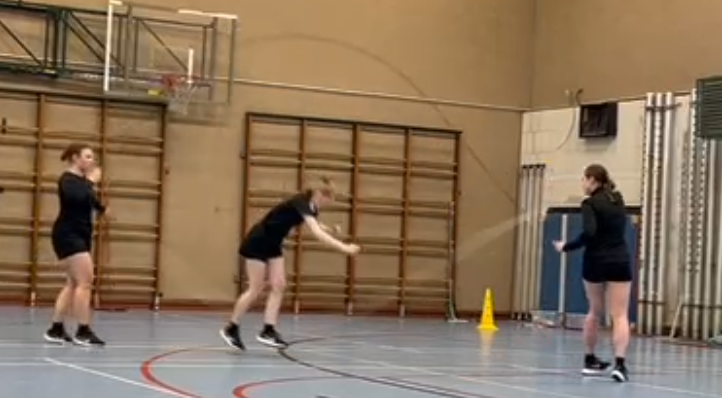
\includegraphics[height=0.14\linewidth]{dd3-du-flip-ts-1}
    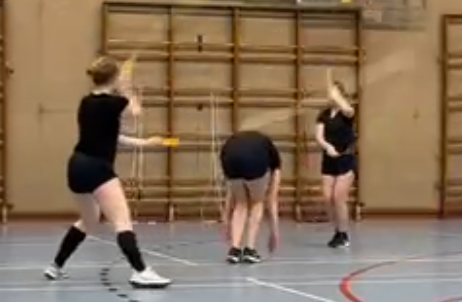
\includegraphics[height=0.14\linewidth]{dd3-du-crab-cross-1}
    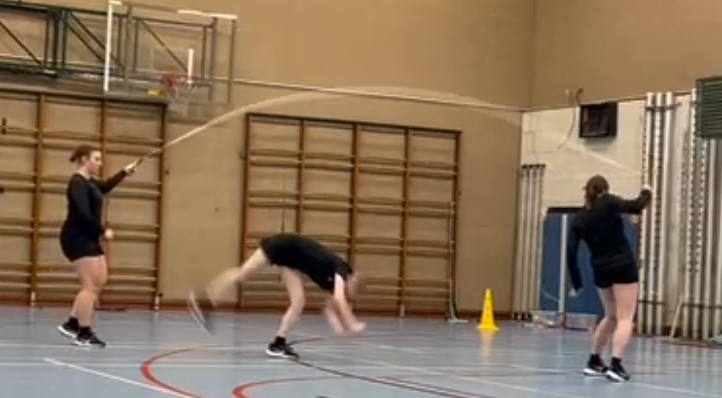
\includegraphics[height=0.14\linewidth]{dd3-du-flip-ts-2}
    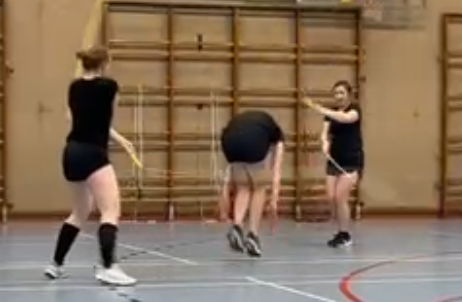
\includegraphics[height=0.14\linewidth]{dd3-du-crab-cross-2}
    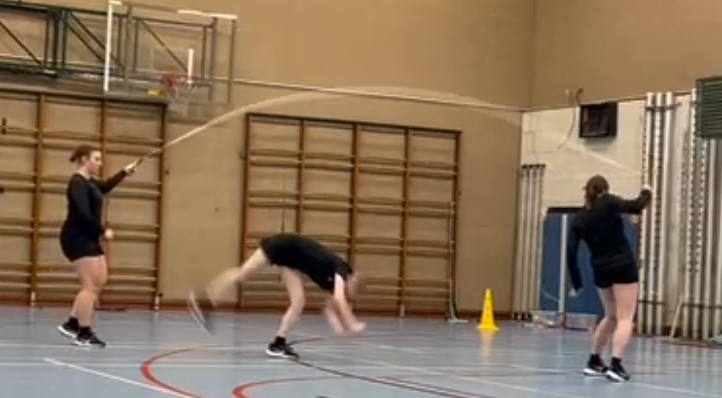
\includegraphics[height=0.14\linewidth]{dd3-du-flip-ts-2}
    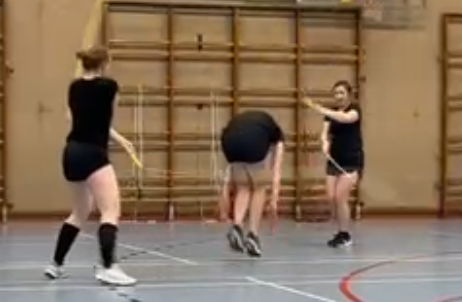
\includegraphics[height=0.14\linewidth]{dd3-du-crab-cross-2}
    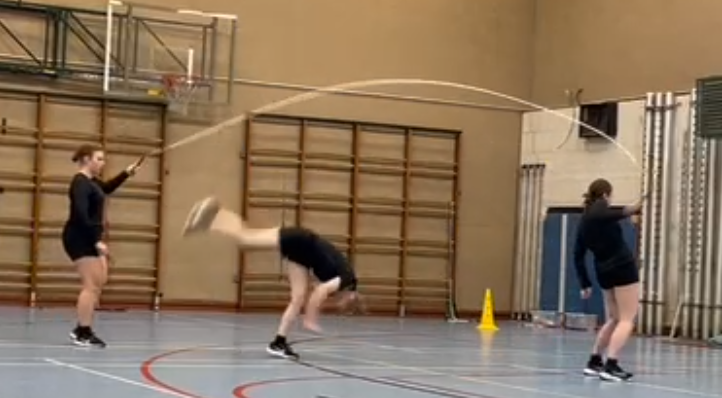
\includegraphics[height=0.14\linewidth]{dd3-du-flip-ts-3}
    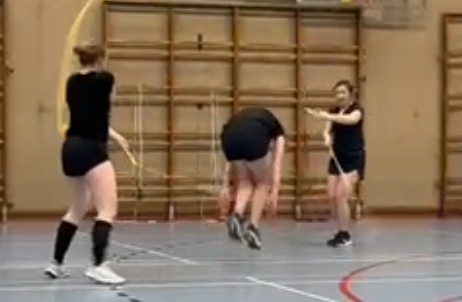
\includegraphics[height=0.14\linewidth]{dd3-du-crab-cross-3}
    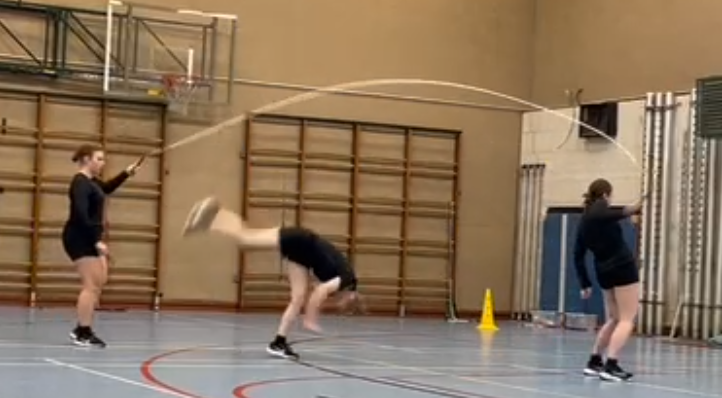
\includegraphics[height=0.14\linewidth]{dd3-du-flip-ts-3}
    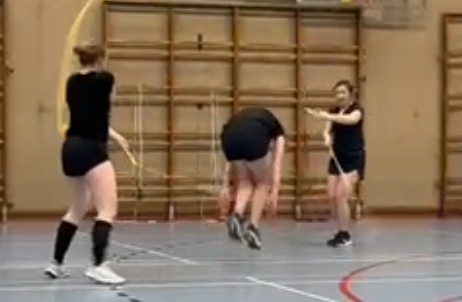
\includegraphics[height=0.14\linewidth]{dd3-du-crab-cross-3}
    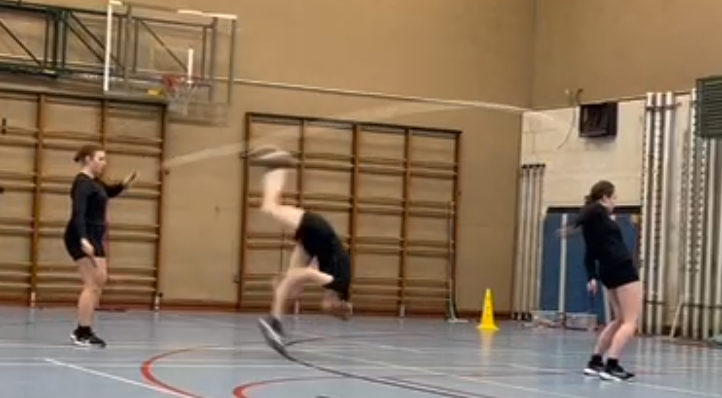
\includegraphics[height=0.14\linewidth]{dd3-du-flip-ts-4}
    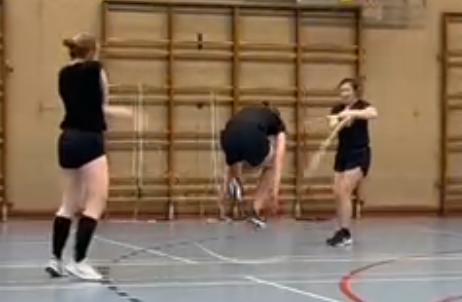
\includegraphics[height=0.14\linewidth]{dd3-du-crab-cross-4}
    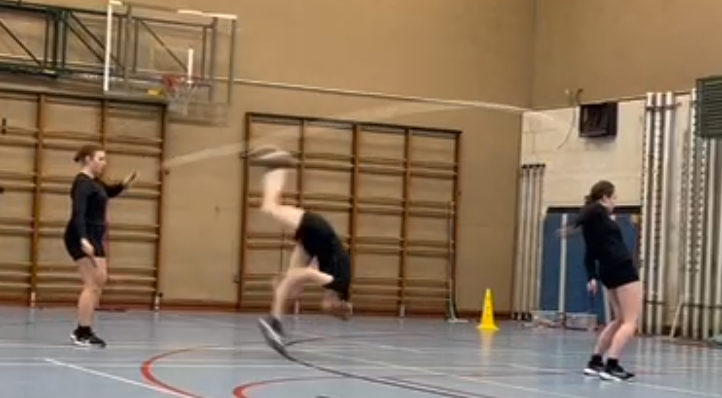
\includegraphics[height=0.14\linewidth]{dd3-du-flip-ts-4}
    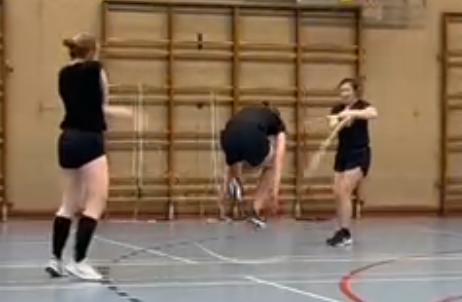
\includegraphics[height=0.14\linewidth]{dd3-du-crab-cross-4}
    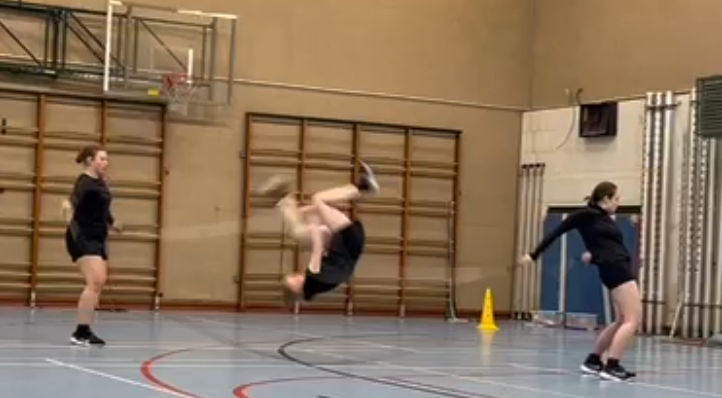
\includegraphics[height=0.14\linewidth]{dd3-du-flip-ts-5}
    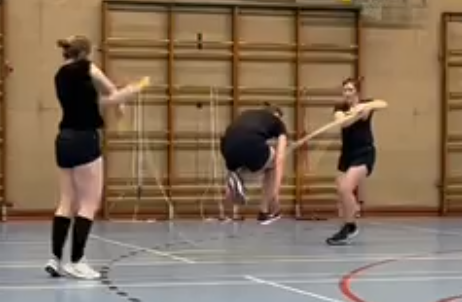
\includegraphics[height=0.14\linewidth]{dd3-du-crab-cross-5}
    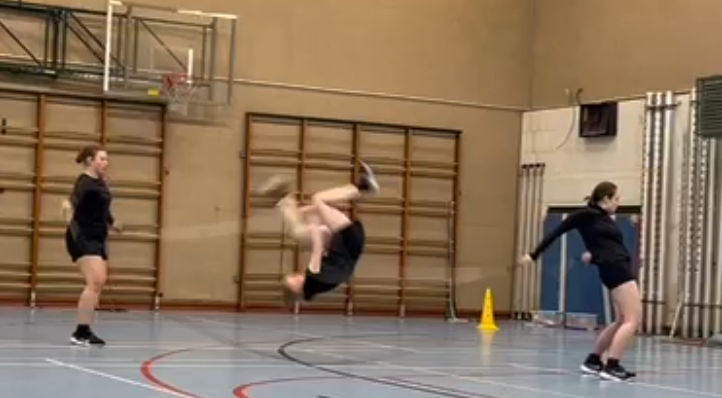
\includegraphics[height=0.14\linewidth]{dd3-du-flip-ts-5}
    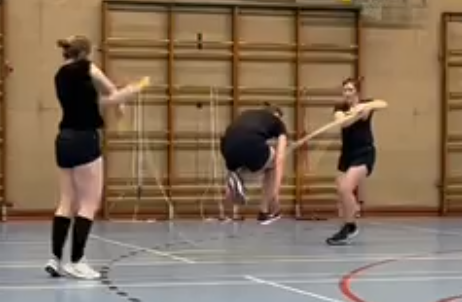
\includegraphics[height=0.14\linewidth]{dd3-du-crab-cross-5}
    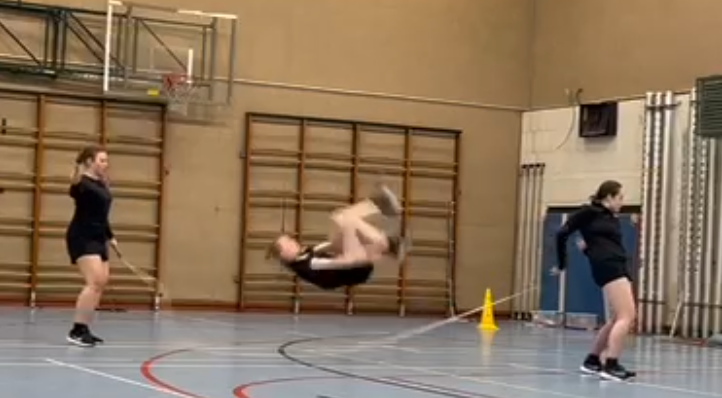
\includegraphics[height=0.14\linewidth]{dd3-du-flip-ts-6}
    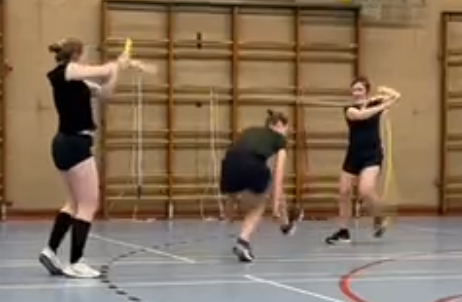
\includegraphics[height=0.14\linewidth]{dd3-du-crab-cross-6}
    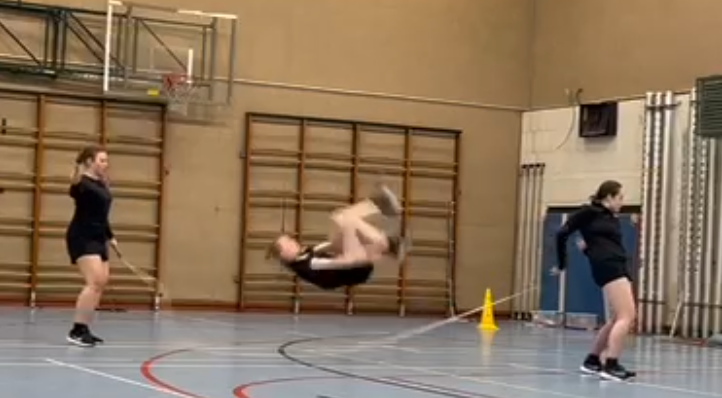
\includegraphics[height=0.14\linewidth]{dd3-du-flip-ts-6}
    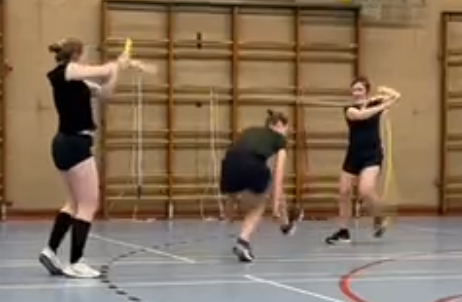
\includegraphics[height=0.14\linewidth]{dd3-du-crab-cross-6}
    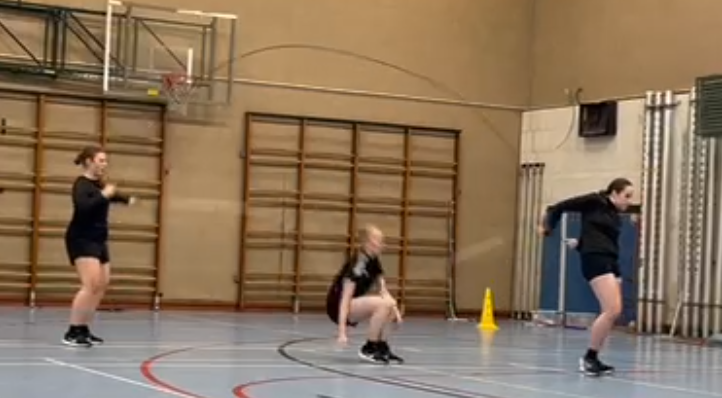
\includegraphics[height=0.14\linewidth]{dd3-du-flip-ts-7}
    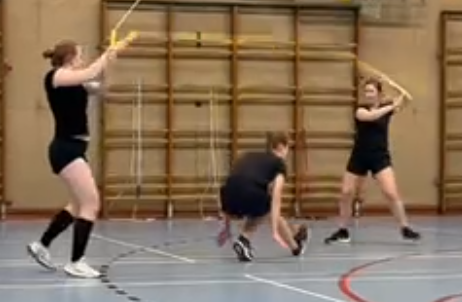
\includegraphics[height=0.14\linewidth]{dd3-du-crab-cross-7}
    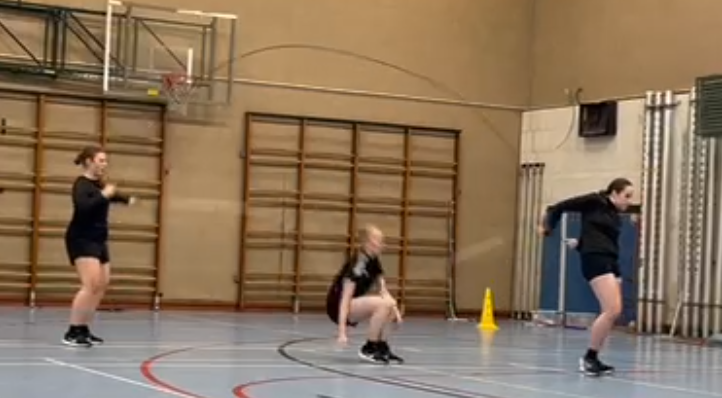
\includegraphics[height=0.14\linewidth]{dd3-du-flip-ts-7}
    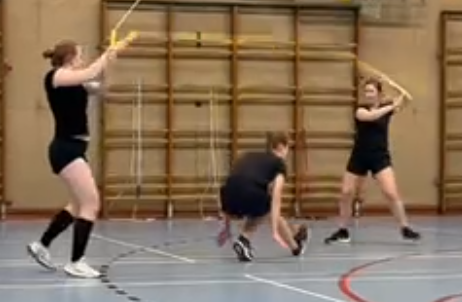
\includegraphics[height=0.14\linewidth]{dd3-du-crab-cross-7}
    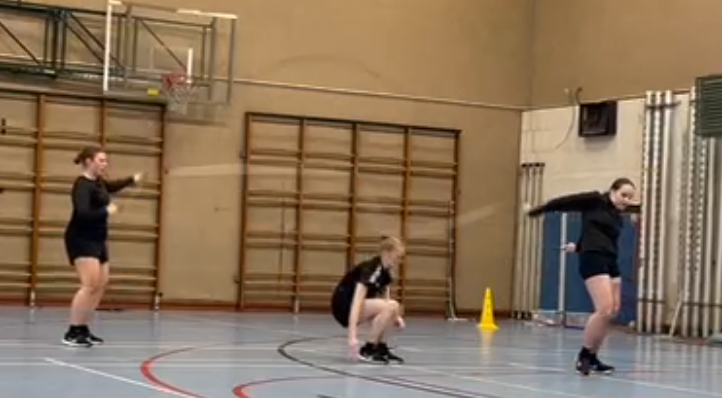
\includegraphics[height=0.14\linewidth]{dd3-du-flip-ts-8}
    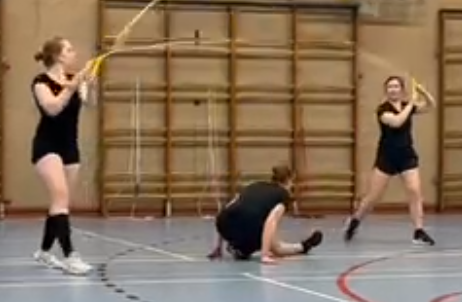
\includegraphics[height=0.14\linewidth]{dd3-du-crab-cross-8}
    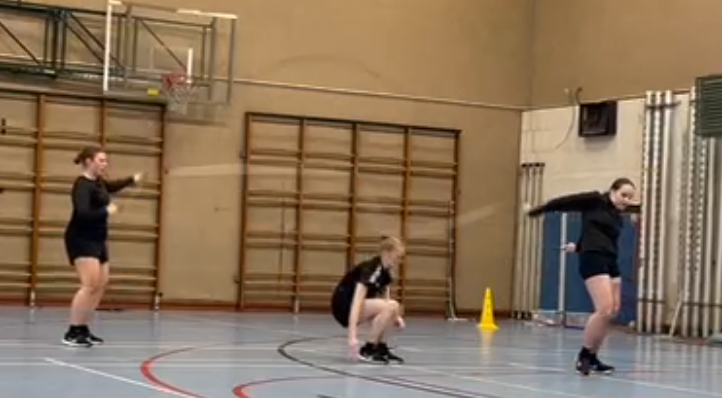
\includegraphics[height=0.14\linewidth]{dd3-du-flip-ts-8}
    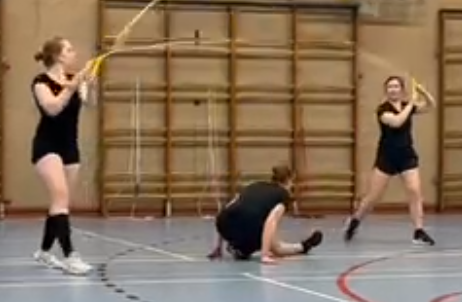
\includegraphics[height=0.14\linewidth]{dd3-du-crab-cross-8}
    \label{fig:skills}
    \caption[DD3 skill flows]{
        Display of 4 skills (currently only 2, 2 others will be added later) \\
        1: A flip while with double under and a TS restriction. \\
        2: A double under with two crosses, while the jumper lands in a crab position. \\
        3: Currently a duplicate of 1 \\
        4: Currently a duplicate of 2 \\
    }
\end{figure}